\newpage
{\bfseries МРНТИ 20.15.05}
\hfill {\bfseries \href{https://doi.org/10.58805/kazutb.v.2.23-429}{https://doi.org/10.58805/kazutb.v.2.23-429}}

\sectionwithauthors{Л.Т. Кусепова, А.Б. Оспанова, А.Е. Назырова, Г.Т. Кусепова}{РАЗВЕРТЫВАНИЕ КОНТЕЙНЕРНЫХ ПРИЛОЖЕНИЙ С ПОМОЩЬЮ МАШИННОГО ОБУЧЕНИЯ: ОБЗОР И АНАЛИЗ}

\begin{center}
{\bfseries \textsuperscript{1,2}Л.Т. Кусепова\envelope, \textsuperscript{1}А.Б.
Оспанова, \textsuperscript{1,2}А.Е. Назырова, \textsuperscript{2}Г.Т.
Кусепова}

\textsuperscript{1}Международный университет Астана, Астана, Казахстан,

\textsuperscript{2}Евразийский национальный университет им. Л.Н.
Гумилева, Астана, Казахстан,

e-mail: lazzatk@mail.ru
\end{center}

В связи с динамическим развитием и растущей сложностью систем необходимо
постоянно выполнять поиск новых методов управления сервисами в облачных
вычислениях. Следовательно технологии контейнеризации помогают легко
развертывать приложения, управлять и распределять ресурсы облачных
провайдеров, тем самым масштабируя их, обеспечивать переносимость данных
и изоляцию приложений и их зависимостей. Однако с ростом сложности
инфраструктуры и данных возникают новые вызовы, такие как обеспечение
непрерывной работы сервисов, оптимизации ресурсов, балансировки
нагрузки, производительности систем. Для решения множеств проблем,
возникающих в контексте развертывания и управления контейнерными
приложениями, становится необходимым применение машинного обучения.
Интеграция технологии контейнеризации и машинного обучения позволяет
адаптироваться к изменяющимся условиям, оптимизировать использование
ресурсов и обеспечивать непрерывную работу системы. В статье представлен
обзор популярных методов машинного обучения и их применение в контексте
контейнерных технологий, была представлена эталонная архитектура
оркестровки контейнеров на основании машинного обучения и их эволюция, а
также были исследованы контейнеры и оркестраторы, такие как Kubernetes,
Docker, Prefect, Nomad, Red Hat OpenShift Service on AWS, Amazon Elastic
Container Service (ECS), Google Kubernetes Engine, Azure Kubernetes
Service. Методы машинного обучения могут быть использованы для
прогнозирования потребления ресурсов, адаптации к потребностям,
предсказания временных интервалов для управления кластерами контейнеров,
а также для анализа поведения рабочей нагрузки на основании прошлых
данных.

{\bfseries Ключевые слова:} контейнерные технологии, оркестровка
контейнеров, машинное обучение, облачные вычисления, предоставление
ресурсов

\begin{center}
{\large\bfseries КОНТЕЙНЕРЛІК ҚОСЫМШАЛАРДЫ МАШИНАЛЫҚ ОҚЫТУ АРҚЫЛЫ ЖҮЗЕГЕ АСЫРУ:
ШОЛУ ЖӘНЕ ТАЛДАУ}

{\bfseries \textsuperscript{1,2}Л.Т. Кусепова\envelope, \textsuperscript{1}А.Б.
Оспанова, \textsuperscript{1,2}А.Е. Назырова, Г.Т.
Кусепова\textsuperscript{2}}

\textsuperscript{1}Астана халықаралық университеті, Астана, Қазақстан,

\textsuperscript{2}Л.Н. Гумилев атындағы Еуразия ұлттық университеті,
Астана, Қазақстан,

e-mail: lazzatk@mail.ru
\end{center}

Жүйелердің динамикалық дамуы мен күрделілігінің артуына байланысты
бұлтты есептеулерде қызметтерді басқарудың жаңа әдістерін үнемі
іздестіріп отыру қажет. Сәйкесінше контейнерлік технологиялар
қолданбаларды оңай орналастыруға, бұлттық провайдер ресурстарын
басқаруға және үлестіруге көмектеседі, осылайша оларды масштабтайды,
деректердің тасымалдануын қамтамасыз етеді және қосымшалар мен олардың
тәуелділіктерін оқшаулайды. Дегенмен, инфрақұрылым мен деректердің
күрделене түсуіне байланысты қызметтердің үздіксіз жұмысын қамтамасыз
ету, ресурстарды оңтайландыру, жүктемені теңестіру және жүйе өнімділігі
сияқты жаңа міндеттер туындайды. Контейнерлік қосымшаларды орналастыру
және басқару контекстінде туындайтын көптеген мәселелерді шешу үшін
машиналық оқытуды пайдалану қажет болады. Контейнерлеу технологиясы мен
машиналық оқытудың интеграциясы өзгермелі жағдайларға бейімделуге,
ресурстарды пайдалануды оңтайландыруға және жүйенің үздіксіз жұмысын
қамтамасыз етуге мүмкіндік береді. Мақалада танымал машиналық оқыту
әдістеріне шолу және оларды контейнерлік технологиялар контекстінде
пайдалану, машиналық оқыту және олардың эволюциясы негізінде
контейнерлік оркестрлеудің анықтамалық архитектурасы ұсынылған, сонымен
қатар Kubernetes, Docker, Prefect, Nomad, Red Hat OpenShift Service on
AWS, Amazon Elastic Container Service (ECS), Google Kubernetes Engine,
Azure Kubernetes Service сияқты контейнерлер мен оркестраторлар
зерттелген. Машиналық оқыту әдістерін ресурстарды тұтынуды болжау,
сұранысқа бейімделу, контейнерлік кластерлерді басқару уақытын болжау
және тарихи деректер негізінде жұмыс жүктемесінің әрекетін талдау үшін
пайдалануға болады.

{\bfseries Түйін сөздер:} контейнерлік технологиялар, контейнерлерді
оркестрлеу, машиналық оқыту, бұлтты есептеулер, ресурстарды ұсыну

\begin{center}
{\large\bfseries DEPLOYING CONTAINER APPLICATIONS THROUGH MACHINE LEARNING:
REVIEW AND ANALYSIS}

{\bfseries \textsuperscript{1,2}L.T. Kussepova\envelope, \textsuperscript{1}A.B.
Ospanova, \textsuperscript{1,2} A.E. Nazyrova, \textsuperscript{2}G.T.
Kussepova}

\textsuperscript{1}Astana International University, Astana, Kazakhstan,

\textsuperscript{2} L.N. Gumilyov Eurasian National University, Astana,
Kazakhstan,

e-mail: lazzatk@mail.ru
\end{center}

Due to the dynamic development and growing complexity of systems, it is
necessary to constantly search for new methods for managing services in
cloud computing. Consequently, containerization technologies help to
easily deploy applications, manage and distribute cloud provider
resources, thereby scaling them, ensure data portability and isolate
applications and their dependencies. However, with the growing
complexity of infrastructure and data, new challenges, such as ensuring
continuous operation of services, resource optimization, load balancing,
and system performance, arise. The use of machine learning becomes
necessary to solve the many problems that arise in the context of
deploying and managing containerized applications. The integration of
containerization technology and machine learning allows you to adapt to
changing conditions, optimize the use of resources and ensure continuous
operation of the system. The article provides an overview of popular
machine learning methods and their application in the context of
container technologies, presented a reference architecture for container
orchestration based on machine learning and their evolution, and also
explored containers and orchestrators such as Kubernetes, Docker,
Prefect, Nomad, Red Hat OpenShift Service on AWS, Amazon Elastic
Container Service (ECS), Google Kubernetes Engine, Azure Kubernetes
Service. Machine learning techniques can be used to predict resource
consumption, adapt to demand, predict timing for managing container
clusters, and analyze workload behavior based on historical data.

{\bfseries Keywords:} container technologies, container orchestration,
machine learning, cloud computing, provision of resources

\begin{multicols}{2}
{\bfseries Введение.} Облачные технологии основаны на аспектах
виртуализации, такие как виртуализация серверов, сети, хранилища данных,
операционной среды и приложений, а также контейнеризация играют ключевую
роль в работе облачных вычислений. Технологии виртуализации и
контейнеризации позволяют предоставлять облачным провайдерам средства
для эффективного управления ресурсами, развертыванием и масштабированием
приложений в облачной среде. Контейнерные технологии обеспечивают
переносимую единицу, которые могут быть легко перенесены и запущены в
различных облачных и локальных средах, тем самым упрощая управление
приложениями и снижая риск возникновения проблем из-за различий в
окружениях.

С динамичным развитием облачных технологий возрастает необходимость
эффективно управлять виртуализацией инфраструктуры и контейнеризацией
приложений. С появлением все более сложных и динамичных приложений, а
также с увеличением требований к производительности и надежности системы
возникает необходимость в поиске новых подходов в предоставлении
сервисов. Соответственно рассмотрение этих аспектов поможет понять каким
образом машинное обучение может повлиять на эффективность создания и
развертывания контейнерных приложений, управления облачными средами и
зависимостями между компонентами приложений.

В нынешнее время машинное обучение стали применяться широкому спектру
задач в различных областях и сферах деятельности, например, при
классификации и кластеризации, в обработке естественного языка, для
распознавания образов и речи, в задачах регрессии, автоматизации
процессов, управления рисками, принятия решений, обнаружения аномалии,
предотвращении сбоев в работе приложений, а также в сфере медицины,
логистики, финансов, Интернет вещей и т.д.

В данной статье будут рассмотрены различные подходы, разработанные в
этой области за последние годы по развертыванию контейнеров,
проанализированы текущие проблемы, с которыми в нынешнее время
сталкиваются системы оркестрации контейнеров.

Оркестровка контейнеров дает возможность поставщикам облачным услуг
легко настраивать, развертывать и обслуживать контейнерные приложения в
облачных вычислениях. На рисунке 1 показана схема архитектуры
оркестровки контейнеров на основе машинного обучения.
\end{multicols}

\begin{figure}[H]
	\centering
	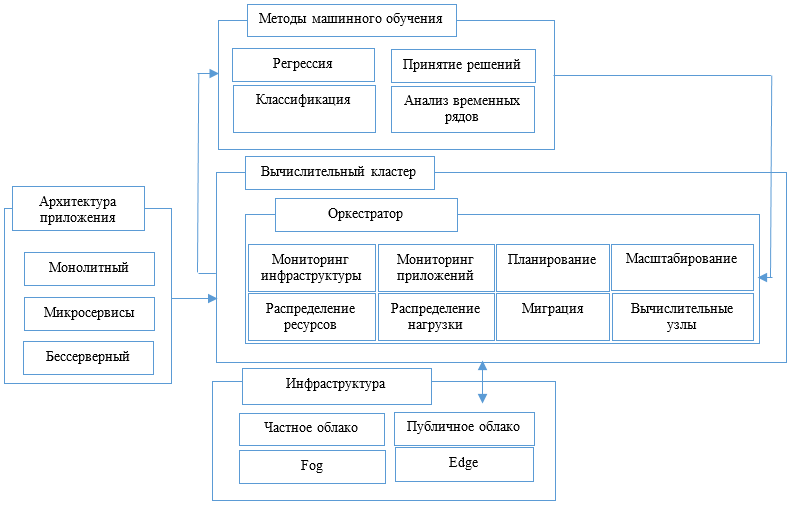
\includegraphics[width=0.8\textwidth]{assets/1000}
	\caption*{Рис. 1 - Эталонная архитектура оркестровки контейнеров на основе машинного обучения}
\end{figure}

\begin{multicols}{2}
В разделе архитектура приложения рисунка 1 представлены наиболее
распространенные и определяющие состав контейнерные приложения, способы
их развертывания, выполнения и обслуживания. Функциональные модули
монолитных приложений разрабатываются и настраиваются в один контейнер,
но при увеличении его масштабов и непрерывном развертывании затраты на
обслуживание могут возрасти. Следовательно, масштабирование монолитного
приложения приведут к снижению общей эффективности и надежности
ресурсов. При разработке приложения с микросервисной архитектурой
функционал разбивается на несколько слабосвязанных и автономных
микросервисных компонентов. Каждый микросервис может быть развернут и
эксплуатироваться независимо друг от друга по различным функциям и
бизнес-целям, однако они могут взаимодействовать между собой и работать
как единое приложение. Структура оркестровки для микросервисной
архитектуры должна обеспечивать поддержку нескольких частей приложения с
соблюдением контроля качества предоставляемых услуг. И для решения такой
проблемы можно применить подходы на основе машинного обучения, чтобы
анализировать зависимости между различными микросервисами и использовать
ресурсы изолированными микросервисами. Бессерверная архитектура
основывается на выполнении вычислительных задач без сохранения состояния
и использования бессерверных функций.

Также на данном рисунке приведены главные методы машинного обучения,
которые применимы в области оркестрации контейнеров. К популярным
алгоритмам регрессии относится регрессия опорных векторов (SVR),
случайный лес, полиномиальная регрессия, Lasso регрессия, Гауссов
процесс, Nearest Neighbor, дерево решений. Методы классификации
применяется в основном для обнаружения аномального поведения и анализа
зависимостей. К нему относится K-means, наивный Байес, машина опорных
векторов, сверточная нейронная сеть. Например, машину опорных векторов
можно использовать для декомпозиции внутренней структуры контейнеров и
K-means для выявления аномального поведения компонентов системы. При
использовании метода принятия решений можно моделировать процесс
принятия решений и определить варианты. Походы обучение с подкреплением
и Марковский процесс принятия решений могут использоваться при выделении
ресурсов каждому контейнеру и масштабировать их в зависимости от
нагрузки, а также автоматизировать процесс развертывания контейнерных
приложений и оптимизировать при управлении ими.

{\bfseries Материалы и методы.} Целью данной статьи является исследование
существующих подходов по развертыванию контейнеров с использованием
методов машинного обучения, рассмотреть их интеграцию, проанализировать
и выявить перспективы их развития. Оценка процесса управления
контейнерными технологиями с применением машинного обучения требовало
выполнения обоснованных исследований алгоритмов регрессии, методов
классификации, моделей принятия решений, анализа временных рядов.
Соответственно в статье предлагается комплексный подход, ориентированный
на достижение цели, включающий следующие этапы и задачи:

- Обзор литературы и сбор данных по контейнерной оркестрации на основе
машинного обучения. На данном этапе будет проведен систематический обзор
существующих контейнерных инструментов с акцентом на использование
методов машинного обучения, включающий в себя анализ научных статей и
публикаций, докладов конференций и исследовательских работ.

- Анализ эволюции технологий. Исследование применения технологии
контейнеров с машинным обучением за период с 2017 года по 2023 год.
Данный этап включает анализ важнейших инноваций и подходов, а также
выявление проблем, с которыми соприкасаются разработчики и
исследователи.

- Исследование современных контейнерных технологий на основе машинного
обучения.

\emph{Литературный обзор}

\emph{Потребности развертывания и управления контейнерными технологиями
на основе машинного обучения}

Алгоритмы регрессии дают возможность спрогнозировать значение выходных
данных посредством анализа связи между выходными и входными данными.
Регрессия опорных векторов, случайный лес и полиномиальная регрессия
используются для понимания и изучения связи между различными
показателями производительности. Например, в работе {[}1{]} проводились
эксперименты по определению влияния конфигурации нескольких Docker
контейнеров и взаимодействия ресурсов на производительность приложений,
а после нескольких экспериментов, была предложена модель прогнозирования
производительности, основанная на регрессии опорных векторов, которая
ориентирована на прогнозирование производительности приложений с
различными настройками и конфигурациями.

Ye K. и др. {[}2{]} провели ряд экспериментов по изучению проблем
надежности облачных систем, основанные на контейнерах, внедрив программы
видов атак на процессор, на память, на диск и DDoS в Docker-контейнер. В
Docker-контейнер установлена среда глубокого обучения TensorFlow и
работают приложения искусственного интеллекта CNN, RNN, BRNN и DRNN. В
результате они разработали модель, обнаруживающий потенциальные
неисправности в контейнерах на основе метода квантильной регрессии.

Следующая работа {[}3{]} ориентирована на изучение влияния ключевых
параметров распределения ресурсов контейнера на производительность
контейнерных приложений. Для многомерного моделирования ресурсов
центрального процессора, памяти и ввода-вывода были использованы три
метода машинного обучения, такие как линейная регрессия, методы опорных
векторов и искусственная нейронная сеть. Потом были оценены методы
моделирования для четырех сложных тестовых рабочих нагрузок от Spark. По
результатам этой исследовательской работы они сделали заключение, что у
моделей с применением опорных векторов и искусственной нейронной сети
точность прогнозирования выше, чем у подходов линейной регрессии.

В статье {[}4{]} были исследованы использование алгоритмов машинного
обучения, такие как многомерные сплайны адаптивной регрессии, методы
повышения (boosting methods), градиентный бустинг, деревья решений,
случайный лес, а также шесть различных приложений и тестов с высокой
активностью ввода и вывода данных, проанализированы точность
прогнозирования, кривую обучения, время обучения и важность функций
алгоритмов на четырех различных моделях SSD с целью предоставления
поставщикам облачных услуг информации по внедрению алгоритмов размещения
контейнеров, совместимых с SLO, на твердотельных накопителях.

В исследовании {[}5{]} предложен подход, основанный на машинном обучении
для автомасштабирования Docker контейнеров при изменении рабочей
нагрузки в реальном времени. Эта архитектура автомасштабирования
включает четыре этапа, такие как мониторинг, анализ, планирование и
выполнение цикла управления. На этапе анализа были использованы
адаптивная и точная модель прогнозирования, основанная на нейронной сети
с краткосрочной памятью, чтобы определить количество контейнеров при
прогнозировании будущей рабочей нагрузки. Экспериментальные результаты
показывают, что точность прогнозирования модели LSTM такая же точная,
как и модель скользящего среднего, интегрированная с авторегрессией. В
ходе исследования было замечено то, что при использовании LSTM
прогнозируемая рабочая нагрузка помогает использовать минимальное
количество реплик для обработки будущей рабочей нагрузки.

В работе {[}6{]}, авторами, которых являются Doukha R. и другие
применили глубокое обучение с классификацией изображений и локализацией
объектов для автоматического развертывания приложений с использованием
современных контейнеров, инструментов развертывания приложений и
оркестрации контейнеров, такие как, Docker, Kubernetes, Ansible и Slurm.

Shahriar H. и другие исследователи {[}7{]} представили обзор
практической лаборатории, в котором применен алгоритм логистической
регрессии для прогнозирования мошенничества с кредитными картами.

\emph{Исследование технологий оркестрации контейнеров, основанный на
машинном обучении в облачных вычислениях}

Оркестрация контейнеров ориентирована на управление и координацию
развертывания контейнеризованными приложениями, позволяют
автоматизировать процессы развертывания и обновления приложений,
оптимизацию и эффективное использование ресурсов, учитывающий текущую
нагрузку, обеспечивающий связь между контейнерами и сетевыми службами,
осуществляющий масштабирование при росте их использования, а также
балансировку нагрузки. Соответственно в данной главе рассматривается
исследовательские работы по технологиям оркестрации контейнеров с
применением алгоритмов и методов машинного обучения. В статье авторами,
которых является Zhong Zh. и другие {[}8{]} представили классификацию
существующих моделей машинного обучения и схему структуры оркестрации
контейнеров.

Работа Rovnyagin M. и других авторов {[}9{]} посвящена изучению
контейнеризации с Docker и больших систем со многими узлами,
выполняющими огромные вычислительные задачи. В статье предлагается
архитектура системы, решающая проблему оркестрации контейнеров с
методами машинного обучения, учитывающий неравномерность потребления
ресурсов.

В книге {[}10{]} предложены различные варианты представления моделей
машинного обучения и глубокого обучения как веб-сервиса на облачной
платформе Databricks с использованием Flask, Streamlit, а также описаны
процессы развертывания контейнера Docker и системы оркестрации
Kubernetes на Google Cloud Platform.

Bandari V. в своей работе {[}11{]} рассматривает различные применения
искусственного интеллекта в контейнеризации, описывает
автоматизированную оркестровку контейнеров, которая позволяет эффективно
управлять большим количеством контейнеров и микросервисов, обеспечивает
балансировку нагрузки и автоматическое масштабирование контейнеров. К
основным компонентам автоматизированной системы оркестрации контейнеров
относится менеджер контейнеров и менеджер кластера. Менеджер контейнеров
ориентирован на создание контейнеров и получение образов из реестра, а
также управляет всем жизненным циклом контейнеров, а менеджер кластера
отвечает за планирование контейнеров, мониторинг их работоспособности и
автоматический перезапуск их в случае сбоя.

В работе {[}12{]} предлагают модель, которая реализуется на
Docker-файле, затем осуществляется обучение данных алгоритму. Набор
данных считывается и выполняется предварительная обработка данных. С
помощью библиотеки Keras импортируются последовательная модель, слой и
оптимизатор Адама. Для точности показателей используется функции
``binary\_crossentroy'' и adam, первое в качестве функции потерь, а
второй как оптимизатор. Сгенерированная модель достигла 73\% точности,
она обучалась на данных 100 раз.

Ahmad I. и другие авторы {[}13{]} исследовали ландшафт современных
методов планирования контейнеров, классифицировали их на четыре
категории такие, как математическое моделирование, эвристика,
метаэвристика и машинное обучение, затем они для каждого класса
алгоритмов планирования проанализировали ключевые преимущества и
недостатки. В работе были изучены статьи и рассмотрены параметры для
планирования контейнеров, такие как энергия, доступность, использование,
балансировка нагрузки, масштабируемость, расходы и сети.

В данной работе {[}14{]} предлагают подход, который автомасштабирует
контейнеры Docker обеспечивающий эластичность, используя вычислительную
модель IBM, принцип Monitor, Analyze, Plan, Execute, and Knowledge для
обеспечения эластичности, а также прогноз рабочей нагрузки, сделанную
моделью

Экспериментальные исследования Chiang R. {[}15{]} ориентирован на оценку
проблемы размещения контейнеров. По эксперименту производительность
распределенных приложений снижается, если они были размещены с другими
контейнерами, потому что контейнеры агрессивно потребляют ресурсы. Для
решения данной проблемы он предлагает новый планировщик, повышающий
производительность при высоком уровне использования ресурсов. Результаты
предложенного прототипа с алгоритмами кластеризации на основе машинного
обучения повышает производительность распределенных приложений до
14,5\%, в среднем до 12\%.

Проведенные исследования в области оркестрации контейнеров с
использованием методов машинного обучения за последние года показывают
прогресс в оптимизации метрик, эффективно развертывая и масштабируя
приложения, повышая при этом производительность и надежность системы
оркестрации. На основании изученных литератур по контейнеризации и
использования в них методов машинного обучения были сформированы
следующая эволюция технологий приведенные в рисунке 2.
\end{multicols}

\begin{figure}[H]
	\centering
	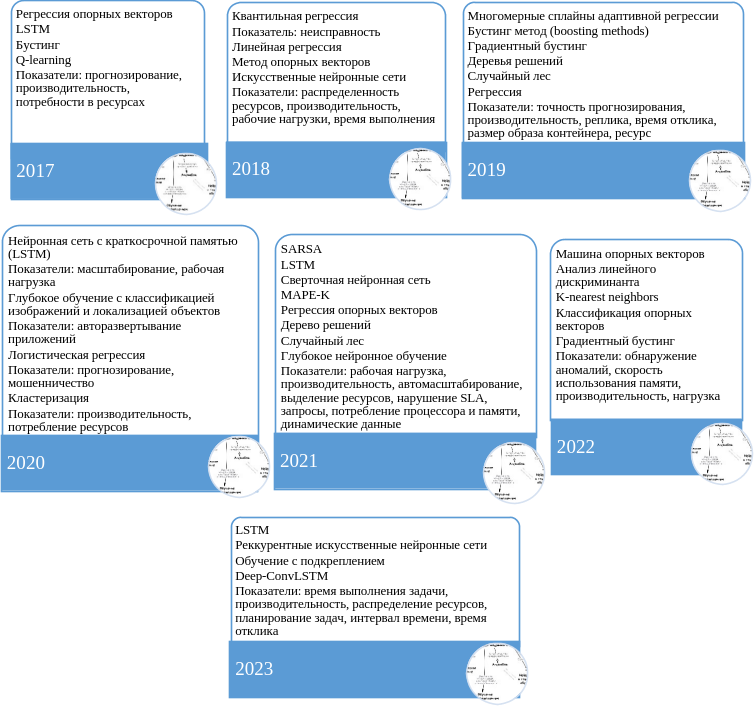
\includegraphics[width=0.8\textwidth]{assets/1001}
	\caption*{Рис. 2 - Эволюция технологий оркестрации контейнеров, используя машинное обучение}
\end{figure}

\begin{multicols}{2}
Проанализировав эволюцию использования машинного обучения в контейнерных
приложениях с 2017 года по 2023 года, можно увидеть разнообразие моделей
и алгоритмов, которые применяются для решения определенных задач, такие
как прогнозирование, оптимизация производительности, управление
ресурсами и т.п. Наряду с этим, прослеживаются и некоторые стабильные
тренды, такие как различные виды регрессии и LSTM. Таким образом,
развитие методов машинного обучения в данной области отражает стремление
к эффективному управлению контейнерными приложениями для улучшения их
надежности и производительности.
\end{multicols}

\begin{table}[H]
\caption*{Таблица 1 - Контейнеры на основе машинного обучения}
\centering
\begin{tabular}{|l|p{0.1\textwidth}|p{0.2\textwidth}|p{0.2\textwidth}|p{0.3\textwidth}|}
\hline
№ & Контейнер & Инструмент оркестрации контейнеров & Компоненты или алгоритм машинного обучения & Источник \\ \hline
1 & Kubernetes & Kubeflow & Библиотеки HuggingFace, DeepSpeed, Megatron-LM & \href{https://www.kubeflow.org/docs/components/training/overview/}{https://www.kubeflow.org} \\ \hline
2 & Kubernetes & Katib & Алгоритмы машинного обучения: Байесовская оптимизация, дерево оценок Парсена, случайный поиск и т.д. & \href{https://www.kubeflow.org/docs/components/katib/overview}{https://www.kubeflow.org} \\ \hline
3 & Docker & Hugging Face Hub & Шаблон Argilla, Livebook & \href{https://www.docker.com/blog/build-machine-learning-apps-with-hugging-faces-docker-spaces/}{https://www.docker.com} \\ \hline
4 & Docker & Datastax & Декларативный язык & \href{https://hub.docker.com/u/datastax?\_gl=1*sbe5u0*\_ga*OTU0NDcxNDk2LjE3MTUzMjQyNzE.*\_ga\_XJWPQMJYHQ*MTcxNTMyNDI3MC4xLjEuMTcxNTMyNDczMC4zOC4wLjA.}{https://hub.docker.com} \\ \hline
5 & Docker & Контейнеры глубокого обучения AWS для PyTorch & SageMaker, EC2, ECS, EKS & \href{https://aws.amazon.com/marketplace/pp/prodview-sdoecebva2lui?sr=0-7\&ref\_=beagle\&applicationId=AWSMPContessa}{https://aws.amazon.com} \\ \hline
6 & Prefect & Prefect & Prefect flow, Prefecr Cloud & \href{https://www.datacamp.com/tutorial/ml-workflow-orchestration-with-prefect}{https://www.datacamp.com} \\ \hline
7 & Nomad & & Плагины устройств и поддержка графических процессоров & \href{https://developer.hashicorp.com/nomad/intro}{https://developer.hashicorp.com} \\ \hline
8 & Red Hat OpenShift Service on AWS & Red Hat OpenShift AI & & \href{https://aws.amazon.com/marketplace/pp/prodview-co7uaxdm7qnkq}{https://aws.amazon.com} \\ \hline
9 & Amazon Elastic Container Service (ECS) & Amazon ECS, Amazon S3 & Библиотека Ray Train & \href{https://aws.amazon.com/ru/blogs/containers/distributed-machine-learning-with-amazon-ecs/}{https://aws.amazon.com} \\ \hline
10 & Google Kubernetes Engine & Kubernetes & PyTorch & \href{ https://cloud.google.com/deep-learning-containers/docs/kubernetes-container}{ https://cloud.google.com} \\ \hline
11 & Azure Kubernetes Service & Kubernetes & AzureML & \href{https://learn.microsoft.com/en-us/azure/machine-learning/how-to-deploy-azure-kubernetes-service?view=azureml-api-1\&tabs=python}{https://learn.microsoft.com} \\ \hline
\end{tabular}
\end{table}

\begin{table}[H]
\caption*{Таблица 2 - Проблемы и решаемые задачи при использовании контейнеров на основе машинного обучения}
\centering
\begin{tabular}{|r|p{0.2\textwidth}|p{0.2\textwidth}|p{0.2\textwidth}|p{0.2\textwidth}|}
\hline
\multicolumn{1}{|l|}{№} & Решаемые задачи & Проблемы и ограничения & Методы & Подходы и типы анализируемых данных \\ \hline
1 & Развертывание приложений с использованием микросервисных приложений и контейнеров Docker & Высокие требования точности и скорости ответа системы & Сверточные нейронные сети, генетические алгоритмы, методы оптимизации, регрессионный анализ & Требования SLA, мониторинг ресурсов, анализ производительности \\ \hline
2 & Планирование задач & Недостаток точности при изменяющихся условиях & Генетические алгоритмы, нейронные сети, методы оптимизации & Анализ загрузки, параметры выполнения, временные рамки выполнения \\ \hline
3 & Размещение контейнеров для кластерных платформ & Планирование компонентов приложения, сложность масштабирования, ограниченные ресурсы & Кластеризация, обучение с подкреплением & Требования SLA, мониторинг ресурсов, анализ производительности \\ \hline
4 & Распределение контейнеров по рабочим узлам и размещение оптимального количества контейнеров на физической машине & Масштабируемость, балансировка нагрузки, анализ ресурсов & Методы оптимизации, алгоритмы распределения ресурсов & Мониторинг ресурсов, анализ производительности \\ \hline
5 & Расширение рабочей нагрузки & Обработка и анализ временных рядов с частотой обновления & Прогнозные модели, нейронные сети, машинное обучение с подкреплением & Исторические данные о нагрузке, производительность \\ \hline
6 & Уменьшение фрагментации сети центров обработки данных и задержка обработки & Сложность в обработке больших объемов данных в реальном времени & Регрессионный анализ, машинное обучение с подкреплением, методы оптимизации & Сетевой трафик, время отклика, статистика потерь пакетов \\ \hline
7 & Частота отказов физических узлов & Высокая стоимость обслуживания, недостаточная надежность & Методы обнаружения аномалий, алгоритмы мониторинга & Мониторинг состояния системы \\ \hline
8 & Динамическая адаптация количеств активных узлов & Отсутствие эффективных механизмов автоматического масштабирования & Алгоритмы масштабирования & Распределение ресурсов и их ограничение, балансировка нагрузки \\ \hline
9 & Временной интервал для выполнения задач размещения и миграции контейнера & Увеличение времени отклика, затраты на выделение ресурсов & Регрессионный анализ & Анализ нагрузки \\ \hline
10 & Оптимизация использования времени и ресурсов & Неэффективное распределение задач & Методы оптимизации, алгоритмы планирования & Анализ загрузки и производительности \\ \hline
\end{tabular}
\end{table}

\begin{multicols}{2}
{\bfseries Результаты и обсуждение.} Рассмотренные работы демонстрируют
широкий спектр использования инструментов оркестрации контейнеров и
алгоритмов машинного обучения, а также их применимости к конкретным
задачам реализации и управления контейнерных приложений, разработки
более сложных моделей, учитывающие динамические изменения в окружающей
среде. Эти инструменты позволяют предоставлять различные
функциональности, включающие распределенное обучение, управление
ресурсами, мониторинг производительности моделей, обеспечивают гибкость
и масштабируемость систем машинного обучения. Некоторые из них будет
рассмотрена на нижеследующей таблице 1.

Рассмотренные результаты исследования подтверждают актуальность и
важность применения методов машинного обучения в контейнеризации и
оркестрации контейнеров. Одним из ключевых моментов является то, что
эффективная оркестровка контейнеров становится сложной и трудоемкой в
условиях динамичной и разнообразной облачной среды. В таких условиях
методы машинного обучения могут оказаться весьма полезными, так как это
позволяет более точному и автоматизированному управлению приложениями в
контейнерах. Следовательно, постоянное обучение моделей на основе новых
данных и изменяющихся условий требует дальнейших исследований и
разработок.

{\bfseries Заключение.} Контейнеризация и оркестрация контейнеров является
эффективными инструментами для развертывания и управления приложениями.
Однако с растущей сложностью динамических сред, в которых работают
контейнеры, становится необходимым применение машинного обучения для
оптимизации и управления процессов контейнерных приложений. И для
достижения оптимальных результатов необходимо решить ряд вызовов по
обработке больших объемов данных, эффективному управлению сложностью
систем, а также по обеспечению его безопасности и конфиденциальности.
Методы машинного обучения, такие как регрессионный анализ, анализ
временных рядов, классификация и принятие решений помогают решать задачи
при планировании и распределении ресурсов, оптимизации
производительности и отклика системы, обеспечении отказоустойчивости и
масштабировании системы. Например, регрессия может использоваться для
прогнозирования потребления ресурсов контейнерами и приложениями,
предсказания временных интервалов для размещения и миграции контейнеров,
также для управления масштабированием кластеров контейнеров, а
классификация может быть применена для распределения контейнеров по их
потребностям в ресурсах и анализа поведения рабочей нагрузки на основе
прошлых данных. Принятие решений нацелена на адаптацию к изменяющимся
условиям и оптимизации работы кластера, а анализ временных рядов может
помочь при задержке обработки данных и прогнозировании будущих
требований к ресурсам, а также анализе сетевого трафика и выявления
аномалии. Исходя из анализа данных о контейнеризации и использования
методов машинного обучения, можно сделать вывод о том, что они помогают
оперативно реагировать на проблемы и ограничения, позволяют на основании
текущего состояния системы адаптировать нагрузки на инфраструктуру
контейнеров и оптимизировать использование ресурсов.
\end{multicols}

\begin{center}
{\bfseries References}
\end{center}

\begin{noparindent}

1.
Ye K., Ji Y. Performance tuning and modeling for big data applications
in docker containers //2017 International Conference on Networking,
Architecture, and Storage (NAS). - IEEE, 2017. -- P. 1-6.

DOI:10.1109/NAS.2017.8026871

2.
Ye K., Liu Y., Xu G., Xu C. Z. Fault injection and detection for
artificial intelligence applications in container-based clouds //
Cloud Computing--CLOUD 2018: 11th International Conference, Held as
Part of the Services Conference Federation, SCF 2018, Seattle, WA,
USA, June 25--30, 2018, Proceedings 11. - Springer International
Publishing, 2018. - P. 112-127. DOI 10.1007/978-3-319-94295-7\_8

3.
Ye K., Kou Y., Lu C., Wang Y., Xu C.Z. Modeling application
performance in docker containers using machine learning techniques
//2018 IEEE 24th International Conference on Parallel and Distributed
Systems (ICPADS). -- IEEE, 2018. -- P. 1-6. DOI
10.1109/PADSW.2018.8644581

4.
Dartois J.E., Boukhobza J., Knefati A., Barais O. Investigating
machine learning algorithms for modeling ssd i/o performance for
container-based virtualization //IEEE transactions on cloud computing.
- 2019. - Vol. 9(3). -- P. 1103-1116.

5.
Imdoukh M., Ahmad I., Alfailakawi M.G. Machine learning-based
auto-scaling for containerized applications //Neural Computing and
Applications. -- 2020. -- Vol. 32(13). -- P. 9745-9760. DOI
10.1007/s00521-019-04507-z

6.
Doukha R., Mahmoudi S.A., Zbakh M., Manneback P. Deployment of
containerized deep learning applications in the cloud //2020 5th
International Conference on Cloud Computing and Artificial
Intelligence: Technologies and Applications (CloudTech). -- IEEE,
2020. -- P. 1-6. DOI 10.1109/CloudTech49835.2020.9365868

7.
Shahriar H., Qian K., Zhang H. Learning Environment Containerization
of Machine Leaning for Cybersecurity //2020 IEEE 44th Annual
Computers, Software, and Applications Conference (COMPSAC). -- IEEE,
2020. -- С. 1131-1132. DOI 10.1109/COMPSAC48688.2020.0-105

8.
Zhong Z., Xu M., Rodriguez M. A., Xu C., Buyya R. Machine
learning-based orchestration of containers: A taxonomy and future
directions //ACM Computing Surveys (CSUR). -- 2022. -- Vol. 54(10). --
P. 1-35.

9.
Rovnyagin M.M., Hrapov A.S., Guminskaia A.V., Orlov A.P. Ml-based
heterogeneous container orchestration architecture //2020 IEEE
Conference of Russian Young Researchers in Electrical and Electronic
Engineering (EIConRus). - IEEE, 2020. - P. 477-481. DOI
10.1109/EIConRus49466.2020.9039033

10.
Singh P. Deploy machine learning models to production. -Cham,
Switzerland: Springer,2021.

11.
Bandari V. A comprehensive review of AI applications in Automated
Container Orchestration, Predictive maintenance, security and
compliance, resource optimization, and continuous Deployment and
Testing //International Journal of Intelligent Automation and
Computing. -- 2021. -- V. 4 (1). -- P. 1-19.

12.
Chowdary M.N., Sankeerth B., Chowdary C.K., Gupta M. Accelerating the
Machine Learning Model Deployment using MLOps //Journal of Physics:
Conference Series. -- IOP Publishing, 2022. -- Vol. 2327(1). DOI
10.1088/1742-6596/2327/1/012027

13.
Ahmad I., AlFailakawi M. G., AlMutawa A., Alsalman, L. Container
scheduling techniques: A survey and assessment //Journal of King Saud
University-Computer and Information Sciences. -- 2021. -- Vol. 34(7).
-- P. 3934-3947. DOI 10.1016/j.jksuci.2021.03.002

14.
Yadav M. P., Rohit, Yadav D. K. Maintaining container sustainability
through machine learning //Cluster Computing. -- 2021. -- Vol. 24(4).
-- P. 3725-3750. DOI 10.1007/s10586-021-03359-4

15.
Chiang R. C. Contention-aware container placement strategy for docker
swarm with machine learning based clustering algorithms //Cluster
Computing. -- 2020. -- Vol. 26(1). -- P. 13-23.
\end{noparindent}

\emph{{\bfseries Сведения об авторах}}

\begin{noparindent}
Кусепова Л.Т. -Международный университет Астана, Евразийский
национальный университет им.

Л.Н.Гумилева, Астана, Казахстан,
e-mail:lazzatk@mail.ru;

Оспанова А.Б. -Евразийский национальный университет им. Л.Н.Гумилева,
кандидат физико- математических наук, Астана, Казахстан,
e-mail:o.ademi111@gmail.com;

Назырова А.Е.-Международный университет Астана, Евразийский национальный
университет им.

Л.Н.Гумилева, Астана, Казахстан,
e-mail:Ayzhan.nazyrova@gmail.com;

Кусепова Г.Т.-Евразийский национальный университет им. Л.Н.Гумилева,
Астана, Казахстан,

e-mail:gulzat.kussepova@gmail.com
\end{noparindent}

\emph{{\bfseries Information about the authors}}

\begin{noparindent}
Kusepova L.T.- Astana International University, L.N. Gumilyov Eurasian
National University, Astana, Kazakhstan, e-mail:lazzatk@mail.ru;

Ospanova A.B.- L.N. Gumilyov Eurasian National University, candidate of
physical and mathematical sciences, Astana, Kazakhstan, e-mail:
o.ademi111@gmail.com

Nazyrova A.E. - Astana International University, L.N. Gumilyov Eurasian
National University, Astan, Kazakhstan,
e-mail:;Ayzhan.nazyrova@gmail.com;

Kussepova G.T. - L.N. Gumilyov Eurasian National University, Astana,
Kazakhstan, e-mail:

gulzat.kussepova@gmail.com
\end{noparindent}
